\section{基础量子算法}

量子计算理论以量子物理领域的数学物理方法、记号与公式为重要基础;本节将对相关内容进行简单介绍。

\subsection{量子比特}

量子比特(qubit)是量子计算和量子信息的基本概念。在传统计算机中,经典比特以 0 和 1 两种状态存在。而量子比特也有相对应的两种形态,在 Dirac 表示法中记作 $\ket{0},\ket{1}$,任何一个两态的量子系统都可以实现这一点,例如在氢原子中 $\ket{0},\ket{1}$ 可以代表基态和第一激发态,在质子自旋中可以表示任意方向的 $+\frac{1}{2},-\frac{1}{2}$ 分量。与经典比特不同的是,量子比特除了 $\ket{0}$ 和 $\ket{1}$ 态,还可以处于叠加态(superposition);这是 $\ket{0},\ket{1}$ 两态的一个线性组合,可以记为 \begin{align}\begin{aligned}
        \ket{\psi}=\alpha\ket{0}+\beta\ket{1}\text{\quad 或列向量形式\quad}\ket{\psi}=
        \begin{bmatrix}
            \alpha \\\beta
        \end{bmatrix}, 
    \end{aligned}\end{align}
其中 $\alpha,\beta\in\mathbb{R}$ (实际上取值域为 $\mathbb{C}^2$,方便起见,这里首先以实数系作为研究对象)且 $|\alpha|^2+|\beta|^2=1$。

在经典比特意义下,$n$ 个比特可以表示 $2^n$ 种不同的状态,在量子比特意义下也是同理,以 $n=2$ 的情况为例,经典比特有四种情况 $00,01,10,11$,而量子比特则用四个维度 $\ket{00},\ket{01},\ket{10},\ket{11}$ 来表示,可以直接写作两个单量子比特的张量积,例如
\begin{align}\begin{aligned}
        \ket{\psi_1}=\begin{bmatrix}
                         \alpha_1 \\\beta_1
                     \end{bmatrix},
        \ket{\psi_2}=\begin{bmatrix}
                         \alpha_2 \\\beta_2
                     \end{bmatrix}
    \end{aligned}\end{align}
的叠加即为
\begin{align}\begin{aligned}
        \ket{\psi_1\psi_2}=\ket{\psi_1}\tensor\ket{\psi_2}=\alpha_1\alpha_2\ket{00}+\alpha_1\beta_2\ket{01}+\alpha_2\beta_1\ket{10}+\beta_1\beta_2\ket{11}=
        \begin{bmatrix}
            \alpha_1\alpha_2 \\\alpha_1\beta_2\\\beta_1\alpha_2\\\beta_1\beta_2
        \end{bmatrix}.
    \end{aligned}\end{align}
特殊地,长度为 $n$ 的全零量子比特表示为 $0^{\tensor n}$,全一量子比特表示为 $1^{\tensor n}$。

\section{量子比特门}

在经典计算机中,逻辑电路由一系列逻辑门与电路元件构成,图 \ref{fig:and-or-not-gate} 即为熟知的与或非逻辑门的表示,它们之间相互嵌套组合,构成了经典电子计算机的电路体系。

\begin{figure}[htbp]
    \label{fig:and-or-not-gate}  %图片引用标记
    \centering    %居中
    \subfigure[逻辑与门] %第一张子图
    {
        \label{fig:and-gate}
        \begin{minipage}{4cm}
            \centering          %子图居中
            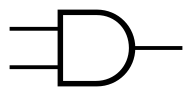
\includegraphics[scale=0.5]{pic/circuit_and.png}   %以pic.jpg的0.5倍大小输出
        \end{minipage}
    }
    \subfigure[逻辑或门] %第一张子图
    {
        \label{fig:or-gate}
        \begin{minipage}{4cm}
            \centering          %子图居中
            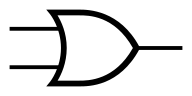
\includegraphics[scale=0.5]{pic/circuit_or.png}   %以pic.jpg的0.5倍大小输出
        \end{minipage}
    }
    \subfigure[逻辑非门] %第一张子图
    {
        \label{fig:not-gate}
        \begin{minipage}{4cm}
            \centering          %子图居中
            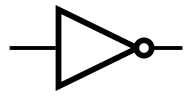
\includegraphics[scale=0.5]{pic/circuit_not.png}   %以pic.jpg的0.5倍大小输出
        \end{minipage}
    }

    \caption{与或非门(ANSI及IEEE标准)} %  %大图名称
\end{figure}

而在量子电路中的计算则由一系列逻辑门、测量与赋值操作构成。但是,不同于传统电路是用金属线所连接以传递电压信号或电流信号;在量子线路中,线路是由时间所连接,亦即量子比特的状态随着时间自然演化,一直到遇上逻辑门而被操作。另一方面,经典计算机的大多数基本逻辑门(除了非门)都是不可逆的,例如,对于与门,我们不可能从输出信息的每一位恢复到两个输入信息;而量子计算中的每一步操作则必须由酉变换(unitary transformation)来刻画\cite{von2018mathematical},变换矩阵 $U$ 满足 $U^\dagger U=I$。下面给出几个基本单量子逻辑门的代数形式。

定义矩阵 $X$ 表示非门 \begin{align}\begin{aligned}
        X=\begin{bmatrix}
              0 & 1 \\
              1 & 0
          \end{bmatrix},\qquad
        \begin{bmatrix}
            \alpha \\\beta
        \end{bmatrix}\mapsto
        \begin{bmatrix}
            \beta \\\alpha
        \end{bmatrix}.
    \end{aligned}\end{align}
显然地,这表示将单量子比特的两位相互交换。这与传统非门是相似的。

定义矩阵 $Z,U$ 表示相位翻转和旋转 \begin{align}
    Z=\begin{bmatrix}
          1 & 0  \\
          0 & -1
      \end{bmatrix}           & ,\qquad
    \begin{bmatrix}
        \alpha \\\beta
    \end{bmatrix}\mapsto
    \begin{bmatrix}
        \alpha \\-\beta
    \end{bmatrix},                      \\
    U=\begin{bmatrix}
          \cos\theta & -\sin\theta \\
          \sin\theta & \cos\theta
      \end{bmatrix} & ,\qquad
    \begin{bmatrix}
        \cos\alpha \\\sin\alpha
    \end{bmatrix}\mapsto 
    \begin{bmatrix}
        \cos(\alpha+\theta) \\\sin(\alpha+\theta)
    \end{bmatrix}.
\end{align}

定义矩阵 $H$ 表示 Hadamard 门 \begin{align}\begin{aligned}
        H=\frac{1}{\sqrt{2}}\begin{bmatrix}
                                1 & 1  \\
                                1 & -1
                            \end{bmatrix}\label{eq:hadamard}
    \end{aligned}\end{align}

考虑将对单量子比特的操作拓展到多量子比特, 我们从一种简单的情况出发。现在有两个量子比特,但是仅对其中的一个,即目标量子比特进行操作,另一个作为控制量子比特,决定是否对目标进行否运算, 于是容易得到这一操作的酉矩阵 \begin{align}\begin{aligned}
        U_{\text{CNOT}}=\begin{bmatrix}
                            1 & 0 & 0 & 0 \\
                            0 & 1 & 0 & 0 \\
                            0 & 0 & 0 & 1 \\
                            0 & 0 & 1 & 0
                        \end{bmatrix}
    \end{aligned}\end{align}
当且仅当控制量子比特为 $1$ 时, 目标量子比特通过非门. 可以被表示为 $\ket{A,B}\to\ket{A,B\xor A}$。因此也被形象地表示为
\begin{figure}[htbp]
    \label{fig:cnot-gate}
    \centering
    \subfigure{
        \begin{minipage}{6cm}
            \centering
            \Qcircuit @C=1em @R=1.2em {
            &\gate{CNOT} & \qw
            }
        \end{minipage}
    }=
    \subfigure {
        \begin{minipage}{6cm}
            \centering
            \Qcircuit @C=1em @R=1.5em {
            &\ctrl{1} & \qw\\
            &\targ & \qw
            }
        \end{minipage}
    }
    =
    \subfigure {
        \begin{minipage}{6cm}
            \centering
            \Qcircuit @C=1em @R=1.2em {
            &\ctrl{1} & \qw\\
            &\gate{X} & \qw
            }
        \end{minipage}
    }
\end{figure}

理论研究证明,任何多量子比特逻辑门可以由受控非门和单量子门组成\cite{},因此,受控非门具有通用性,这也与经典电路中与非门(XAND)的通用性相对应。

\newpage
\subsection*{思考:与线性代数知识的关联}

\subsubsection*{基向量,投影与测量}
在学习量子计算相关入门知识时,笔者发现其与本科一年级所学线性代数知识的高度关联性,这样就能更方便地从向量空间的意义上去理解量子比特了。例如,在常规使用的量子比特基 $\ket{0},\ket{1}$ 下,我们有一个态向量 \begin{align*}
    \ket{\psi}=\alpha\ket{0}+\beta\ket{1}.
\end{align*}
在此前的章节中,我们看到了 $\ket{0},\ket{1}$ 在现实世界中具有的一些物理意义;那么,式子中的系数 $\alpha,\beta$ 又对应了什么含义呢?首先,考虑这个态向量在这组正交基上的投影,这也就是量子力学中的测量过程: \begin{align*}
    \overrightarrow{\psi_0}=(\overrightarrow{0})^{\text{T}}\overrightarrow{\psi}\overrightarrow{0}\Rightarrow\ket{\psi}^{\dagger}\ket{0}\ket{0}=\bra{\psi}\ket{0}\ket{0}=\inner{\psi}{0}\ket{0}=\alpha\ket{0}
\end{align*}
其中,左式是在线性代数中熟知的投影运算形式 $\bm{p}=\bm{u}^{T}\bm{v}\bm{u}$,右式是在量子力学中用 Dirac 记号刻画的更加优美的形式,其中将 $\ket{\psi}^\dagger$ 改写为 $\bra{\psi}$,进而将 $\ket{\psi}\cdot\ket{0}$ 缩写为 $\inner{\psi}{0}$,再考虑投影向量长度的平方 \begin{align*}
    \alpha\bra{0}\cdot\alpha\ket{0}=\alpha^2.
\end{align*}
而在 $\ket{1}$ 上的分量长度平方同理则为 $\beta^2$,这样一来,约束条件 $\alpha^2+\beta^2=1$ 的意义就逐渐清晰:态向量始终在单位圆上运动,被测量时,其落在 $\ket{0},\ket{1}$ 上的概率之和恰好为 $1$.

\subsubsection*{线性变换}
对于一些更加抽象的情况,例如一组新的标准正交基 \begin{align*}
    \ket{+}=\frac{\ket{0}+\ket{1}}{\sqrt{2}},\ket{-}=\frac{\ket{0}-\ket{1}}{\sqrt{2}}
\end{align*}
可以从基变换的角度进行理解。根据基坐标变换的公式,变基矩阵为 \begin{align}\begin{aligned}
    M=\frac{1}{\sqrt{2}}\begin{bmatrix}
        1 & 1\\
        1 & -1
    \end{bmatrix}\label{eq:change-of-basis}
\end{aligned}\end{align}
这是一个标准正交阵(当然,在 $\mathbb{C}^n$ 中应为酉阵,但线性代数课程尚未涉及),便有了 \begin{align*}
    M^{-1}=M=M^{\text{T}}.
\end{align*}
这样的规律还可以推广到更加一般的基变换,例如在随后的公式  中进行的复向量基变换等,对线性代数基础知识的掌握要求较高。

同时,容易观察到,式 \ref{eq:change-of-basis} 与 式 \ref{eq:hadamard} 的形式是相同的,并且有 \begin{align*}
    \frac{1}{\sqrt{2}}\begin{bmatrix}
        1 & 1\\
        1 & -1
    \end{bmatrix}
    \begin{bmatrix}
        \cos\alpha\\
        \sin\alpha
    \end{bmatrix}
    =\begin{bmatrix}
        \cos(\frac{\pi}{4}-\alpha)\\
        \sin(\frac{\pi}{4}-\alpha)
    \end{bmatrix}
\end{align*} 代表了将一个 $\mathbb{R}^2$ 中的向量对 $\theta=\frac{\pi}{8}$ 进行对称,从而将 $\ket{0}$ 映射为 $\ket{+}$,$\ket{1}$ 映射为 $\ket{-}$,这样就能制备出等概率落在 $\ket{0},\ket{1}$ 上的叠加态。

而在从单量子比特到多量子比特的拓展中,



正如在线性代数中对线性映射进行线性变换一样,在量子力学中也可以对量子比特门进行变换,比如通过给单量子比特门 $H$ 进行张量积 $H^{\tensor n}$,就可以制备 $n$ 量子比特的等概率叠加态 \begin{align*}
    H^{\tensor n}(\ket{0}^{\tensor n})=\ket{+}^{\tensor n}.
\end{align*}




\subsection{Deutsch-Jozsa 算法}

Desutsch-Jozsa 算法可由一个简单的游戏进行引入:Alice 从 $0-2^{n}-1$ 中选一个数 $x$ 并将其传送给 Bob。Bob 计算出某个函数 $f(x)$ 的值,可以为 $0$ 或 $1$,并将它传回给 Alice。已知该函数只有可能有两种情况:要么 $f(x)$ 对于所有的 $x$ 均为常数,要么 $f(x)$ 恰好对于一半的 $x$ 取 $0$,一半的取 $1$。Alice 怎样能够最快地判断 $f(x)$ 的类型?

形式化地,已知函数 $f:\{0,1\}^{\otimes n}\rightarrow\{0,1\}$ 一定是下列两种极端形式的一种:
\begin{enumerate}
    \item Constant:$f(x)\equiv 0\text{ or }f(x)\equiv 1$;
    \item Balanced:$f(x)=0~~\text{for half of }\{0,1\}^{\otimes n},\text{ and }f(x)=1~~\text{for the other half}$
\end{enumerate}

问如何用最少的查询次数确定 $f$ 属于二者中的哪一种。

\begin{figure}[htbp]
    \label{fig:deu-joz}
    \centering
    \begin{minipage}{12cm}
        \centering
        \def\ingate{\vbox to 3.5em{\hbox to 4em{\tiny$x$\hss $x$}\vss
                    \hbox to 4em{\Large\hss$U_f$\hss}\vss
                    \hbox to 4em{\medmuskip1mu\tiny$x$\hss $y\oplus f(x)$}\vskip-2pt}}
        \Qcircuit @C=1em @R=2em {
        \lstick{\hbox to 2em{$\ket{0}^{\tensor n}$\hss}} & {/}\qw& \qw & \gate{\hbox{\small$H^{\otimes n}$}} & \multigate{1}{\ingate} & \gate{\hbox{\small$H^{\otimes n}$}} & \qw & \meter \\
        \lstick{\hbox to 2em{$\ket{0}$\hss}} & \qw & \gate{X} & \gate{H} & \ghost{\ingate} & \qw & \qw & \\
        }
    \end{minipage}
    \caption{Deustch-Jozsa 算法的量子电路}
\end{figure}

考虑图 \ref{fig:deu-joz} 所示量子电路,输入 $U_f$ 的初态为 $\ket{+}^{\tensor n}\ket{-}$。考虑初态的前 $n$ 位,设其在某一状态下为 $x$,那么 \begin{align*}
    U_f\ket{x}\ket{-}=\ket{x}\ket{-\tensor f(x)}=(-1)^{f(x)}\ket{x}\ket{-}.
\end{align*}
从而 \begin{align*}
    U_f\ket{+}^{\tensor n}\ket{-}=\sum_{x\in\{0,1\}^{\tensor n}}\frac{(-1)^{f(x)}}{\sqrt{2^n}}\ket{x}\ket{-}.
\end{align*}
另外,容易验证,对于单量子比特门 $H\ket{x}=\sum_{z\in\{0,1\}}(-1)^{xz}\ket{z}/\sqrt{2}$,将这一结果推广到 $n$ 个量子比特上,就有了 \begin{align*}
    H^{\tensor n}\ket{x}=\sum_{z\in\{0,1\}^{\tensor n}}\frac{(-1)^{x\cdot z}}{\sqrt{2^n}}\ket{z}.
\end{align*}
从而 \begin{align*}
    H\left(\sum_{x\in\{0,1\}^{\tensor n}}\frac{(-1)^{f(x)}}{\sqrt{2^n}}\ket{x}\right)=\sum_{x,z\in\{0,1\}^{\tensor n}}\frac{(-1)^{x\cdot z+f(x)}}{2^n}\ket{z}\to\ket{\psi}_{\text{measure}}
\end{align*}
于是考虑测量结果在 $\bra{0^{\tensor n}}$ 上的分量,即 $z$ 只取 $\ket{0}^{\tensor n}$ 时表达式的值 \begin{align*}
    \inner{0^{\tensor n}}{\psi}=\sum_{x\in\{0,1\}^{\tensor n}}\frac{(-1)^{f(x)}}{2^n}
\end{align*}
因此,当 $f$ 为常值函数时,测量结果必为 $\ket{0}^{\tensor n}$;当 $f$ 为平衡函数时,测量结果不可能出现 $\ket{0}^{\tensor n}$.

\subsection{量子傅里叶变换}

在离散傅里叶变换(Discrete Fourier Transform,DFT)中,我们熟知求多项式 $f(x)$ 进行点值 $(\omega_N^k,y_k)$ 求值的方法 \begin{align*}
    y_k=\frac{1}{\sqrt{N}}\sum_{j=0}^{N-1}x_j\omega_N^{jk}.
\end{align*}
在经典计算机中,可以通过分治加速的方式将这一过程(快速傅里叶变换,Fast Fourier Transform)的时间复杂度优化为 $O(n\log n)$\cite{cooley1965algorithm}。在量子计算机中,我们同样希望进行相同的变换,使得 $N-1$ 维量子态 $\ket{X}=\sum_{j=0}^{N-1}x_j\ket{j}$,经过变换得到 $\ket{Y}=\sum_{k=0}^{N-1}y_k\ket{k}$,其中 $y_k$ 与 $x_k$ 的关系满足上式,$\ket{j},\ket{k}$ 表示其二进制分解所得结果的张量积。代入可得 \begin{align*}
    \ket{Y}=\sum_{k=0}^{N-1}y_k\ket{k}=\sum_{k=0}^{N-1}\left(\frac{1}{\sqrt{N}}\sum_{j=0}^{N-1}x_j\omega_N^{jk}\ket{k}\right)=\sum_{j=0}^{N-1}x_j\left(\frac{1}{\sqrt{N}}\sum_{k=0}^{N-1}\omega_N^{jk}\ket{k}\right)
\end{align*}
对比 $\ket{X},\ket{Y}$ 的形式,发现变换的实质就是一次基变换 \begin{align*}
    \ket{j}\to\frac{1}{\sqrt{N}}\sum_{k=0}^{N-1}w_N^{jk}\ket{k}
\end{align*}
两组标准正交基的变换可改写为酉变换 \begin{align*}
    U_{\text{QFT}} = \frac{1}{\sqrt{N}}
    \begin{bmatrix}
        1      & 1               & 1                         & \cdots & 1                      \\
        1      & \omega_N        & \omega_N ^{2}             & \cdots & \omega_N ^{N-1}        \\
        1      & \omega_N ^{2}   & \omega_N ^{4}             & \cdots & \omega_N ^{2(N-1)}     \\
        1      & \omega_N ^{3}   & \omega_N ^{6}             & \cdots & \omega_N ^{3(N-1)}     \\
        \vdots & \vdots          & \vdots                    & \ddots & \vdots                 \\
        1      & \omega_N ^{N-1} & \omega_N ^{(N-1)\times 2} & \cdots & \omega_N ^{(N-1)(N-1)}
    \end{bmatrix}
\end{align*}
更形象化地,考虑直接对 $\omega_{2^n}^{jk}=\exp(\frac{2\pi\i jk}{2^n})$ 指数中的 $\frac{k}{2^n}$ 进行二进制小数分解,也即对 $k$ 进行二进制分解,得到 \begin{align*}
    \ket{j}\to\frac{1}{\sqrt{N}}\sum_{k=0}^{N-1}w_N^{jk}\ket{k}
     & =2^{-\frac{n}{2}}\sum_{l\in[n],k_l\in\{0,1\}}\exp\left(2\pi\i j\left(\sum_{l\in[n]}k_l2^{-l}\right)\right)\ket{k_1,\cdots,k_n} \\
     & =2^{-\frac{n}{2}}\bigotimes_{l\in[n]}\left(\sum_{k_l\in[0,1]}\exp(2\pi\i jk_l2^{-l})\ket{k_l}\right)                           \\
     & =2^{-\frac{n}{2}}\bigotimes_{l\in[n]}\left(\ket{0}+\exp(2\pi\i j2^{-l})\ket{1}\right)                                          \\
     & =2^{-\frac{n}{2}}\bigotimes_{l\in[n]}\left(\ket{0}+\exp(2\pi\i\{j\!>\!\!\!>\!l\})\ket{1}\right)
\end{align*}
这里的 $\{j\!>\!\!\!>\!l\}$ 表示 $j$ 按位右移 $l$ 位并取其小数部分。

\subsection{}

